\chapter{Simulation de l'environnement}
\chaptermark{Environnement}
\label{chapitre:environnement}
	
	\section{Introduction}

		La simulation de l'environnement est une partie importante du simulateur car c'est ce qui va définir le comportement des \gls{ROV}s dans leur milieu. Elle doit être très proche des conditions réelles afin d'avoir des résultats exploitables. A la fin de cette partie, nous devrions avoir à notre disposition un environnement de simulation complet proche de l'environnement rencontré lors de missions avec les robots.

		Il est donc nécéssaire d'établir les différents élements de l'environnement qui vont interagir avec les \gls{ROV}s afin de les intégrer dans le simulateur. Il y a principalement le milieu marin qui va ajouter une flottabilité au robots, les vagues, le vent, mais aussi la présence de courants marins. Ensuite, il y a l'ombilical qui relie les \gls{ROV}s au bateau afin de l'alimenter en énergie mais aussi d'avoir un retour d'informations. Enfin la présence de structures sous-marines jouent aussi un rôle importante dans les missions des \gls{ROV}s, que ce soit par exemple des piles d'éolienne à inspecter pour le robot \gls{Argos}, son garage, ou bien des \gls{frameLBL} à deplacer pour \gls{Atoll}.

		La \textsc{Table}~\ref{table:elements} présente les différents élements cités précédemment qui peuvent être simulés dans un environnement marin. Nous allons choisir les principaux car tous n'auront pas un impact significatif sur le comportement des \gls{ROV}s, comme le vent ou les vagues. 

		\begin{table}[ht]
			\centering
			\begin{tabular}{|c|c|}
				\hline
				\textbf{Elément} & \textbf{Simulation} \\
				\hline
				Vent & \xmark\\
				\hline
				Vagues & \xmark\\
				\hline
				Courant marins & \cmark \\
				\hline
				Ombilical & \cmark \\
				\hline
				Garage d\gls{Argos} & \cmark \\
				\hline
				\gls{frameLBL} & \cmark \\
				\hline
				Pile d'éolienne & \cmark \\
				\hline
			\end{tabular}
			\caption{Elements pris en compte dans l'environnement de simulation}
			\label{table:elements}
		\end{table}

	\section{Simulation d'environnements marins}

		\section{Simulation des courants marins}

			Les courants marins constituent un élément majeur qui va perturber le comportement des robots dans l'environnement simulé. Avec une simulation suffisament précise, la simulation et le comportement réel des \gls{ROV}s deviendront très proches, notamment par l'ajout de la traînée hydrodynamique qui va s'appliquer sur les composants des robots.

			\subsection{Modèle constant}

				Pour simuler ces courants, il est possible d'utiliser en première approximation une idée assez triviale : localement le courant est constant. Par constant on entend uniforme, donc qui ne dépend pas de l'espace, et stationnaire, donc qui ne dépend pas du temps. C'est à dire qu'il serait possible de considérer le courant marin  comme un champ de vecteurs ayant un certain cap et une certaine magnitude représentant la vitesse de l'écoulement. Ce modèle simple permet de rapidement ajouter du courant dans notre simulateur, mais ce courant est peu réaliste dans la mesure ou il ne prends pas du tout en compte la présence de structures sous-marine qui pourraient modifier la vitesse et l'orientation de ce courant.

			\subsection{Modèle procédural}

				Une autre idée serait de générer un courant pseudo-aléatoire par génération procédurale. Cette méthode de génération est largement utilisée dans le domaine des jeux-vidéos et du cinéma, et par extension, il est aussi utilisé dans le domaine de la simulation. Elle permet de générer à l'aide d'algorithme des mondes et des textures pseudo-aléatoires. Dans notre cas, il est possible d'utiliser le \textit{Bruit de Perlin} qui est une texture procédurale. Cette texture se distingue d'une texture complètement aléatoire qui n'est clairement pas esthétique. Une comparaison de ces deux textures est présentée en \textsc{Figure}~\ref{fig:texture}. L'avantage du \textit{Bruit de Perlin} est qu'il est très peu coûteux en espace mémoire et qu'il peut générer des textures dans n'importe quelle dimensions. 
				
				Pour notre application nous pouvons générer une texture en deux dimensions. Cette texture formerait un potentiel artificiel, et un champ de vecteur représentant le courant peut être simplement généré en prenant le gradiant de ce potentiel. On obtient le résultat présenté en \textsc{Figure}~\ref{fig:perlin_noise}. Comme avec cette méthode, chaque pixel tient compte de ses pixels voisins, on ne se retrouve pas avec des valeurs très eloignées entre deux pixels adjacents comme avec de la génération de textures purement aléatoire, et on obtient des courants réalistes. 

			\subsection{Modèle de Navier-Stokes}

				Une simulation des courants marins basée sur les équations de Navier-Stokes permet de proposer une approche intéressante à la simulation de courants marins~\cite{Garau2006current}. Ils permettent notament de générer des courants prenant en compte la présence de solides dans le milieu à explorer, comme des rochers ou des piles d'éoliennes offshores qui peuvent être intéressante pour notre application.

			\subsection{Choix du modèle}

				Il faut maintenant choisir un modèle qui va être implémenté dans le simulateur. Pour nous aider dans ce choix, la \textsc{Table}~\ref{table:courants} reprends les principales caractéristiques des différents modèles. La complexité d'implémentation de la solution est aussi ajoutée. Elle représente à la fois le temps d'implémentation de la solution ainsi que la complexité d'execution de celle-ci en terme de ressources utilisées par le simulateur pour générer et appliquer ces courants marins sur les \gls{ROV}s. Elle est représentée par le symbole \pmark (\pmark : \textit{simple}, \pmark \pmark : \textit{intermédiaire}, \pmark \pmark \pmark : \textit{complexe}).

				\begin{table}[ht]
					\centering
					\begin{adjustbox}{max width=\textwidth}
						\begin{tabular}{|c|c|c|c|c|}
							\hline
							\textbf{Modèle de courants} & \textbf{Aléatoire} & \textbf{Structures sous-marines} & \textbf{Réalisme} & \textbf{Complexité} \\
							\hline
							Modèle constant & \xmark & \xmark & \pmark & \pmark\\
							\hline
							Modèle procédural & \cmark & \xmark & \pmark \pmark & \pmark \pmark\\
							\hline
							Modèle Navier-Stokes & \xmark & \cmark & \pmark \pmark \pmark & \pmark \pmark \pmark \\
							\hline
						\end{tabular}
					\end{adjustbox}
					\caption{Différents modèles de simulation de courants}
					\label{table:courants}
				\end{table}

		\section{Simulation d'ombilicaux}

			\subsection{Etat de l'art}

\subsection{Formalisme}

\subsection{Initialisation}
    L'initialisation des différents n\oe uds de l'ombilical est une étape importante car les coefficients du modèle comportemental sont reglés pour avoir un comportement cohérent lorsque la position du câble a convergée. Si l'initialisation est aléatoire, le temps du régime transitoire peut être long et la simulation peut ne pas être consistante.

    Pour initialiser l'ombilical, nous allons nous appuyer sur l'équation de la chaînette. Cette équation issue du calcul variationnel représente la forme que prend une corde attachée à ses deux extrémités afin de limiter son énergie. La \textsc{Figure}~\ref{fig:chainette} représente un tracé de cette équation.

    \begin{figure}[!htb]
        \centering
        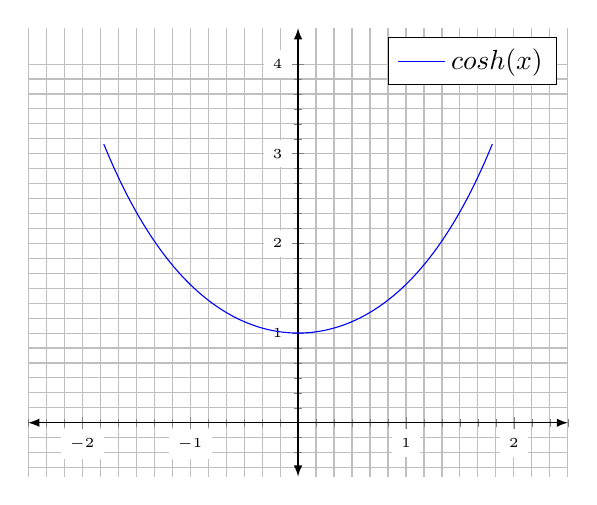
\begin{tikzpicture}
            \begin{axis}[
                    xmin=-2,   xmax=2,
                    ymin=-0.1,   ymax=3.9,
                    grid=both,
                    axis lines=middle,
                    minor tick num=5,
                    enlargelimits={abs=0.5},
                    axis line style={latex-latex},
                    ticklabel style={font=\tiny,fill=white},
                    xlabel style={at={(ticklabel* cs:1)},anchor=north west},
                    ylabel style={at={(ticklabel* cs:1)},anchor=south west}
                ]
                \addplot [
                    domain=-1.8:1.8, 
                    samples=100, 
                    color=blue,
                    ]
                    {cosh(\x)};
                \addlegendentry{$cosh(x)$}
            \end{axis}
        \end{tikzpicture}
        \caption{Représentation graphique de l'équation de la chaînette}
        \label{fig:chainette}
    \end{figure}
    

\subsection{Implémentation}
    L'implémentation d'un \gls{Plugin} \gls{Gazebo} permet de simuler le comportement de l'ombilical dans l'environnement de simulation. Ce \gls{Plugin} est basé sur l'instanciation d'objets de type \textit{Tether} et \textit{TetherElement}. L'objet \textit{Tether} possède les paramètres de simulation de l'ombilical, tandis que l'objet \textit{TetherElement} représente un tronçon de cet ombilical. Un diagramme de classe est présenté en \textsc{Figure}~\ref{fig:uml_class} et montre les différents attributs et méthodes associées à chaque classe.
    
    La \textit{Tether} utilise une structure de liste doublement chaînée\footnote{structure de données liée qui consiste en un ensemble n\oe uds liés les uns aux autres par des références au n\oe uds voisins.} de \textit{TetherElement}. Chaque \textit{TetherElement} possède alors une référence vers l'élément le précédant et l'élément le suivant, comme le montre la \textsc{Figure}~\label{fig:goubly_linked_list}. La \textit{Tether} ne possède ainsi qu'une référence vers le premier et le dernier n\oe ud de la chaîne, nommés respectivements \textit{head} et \textit{tail}. Il est ensuite possible de parcourir la chaîne de \textit{TetherElement} dans les deux sens en utilisant les références gardées par les \textit{TetherElement} eux-mêmes. 

    \begin{figure}[!htb]
        \centering
        \resizebox{0.90\textwidth}{!}{
            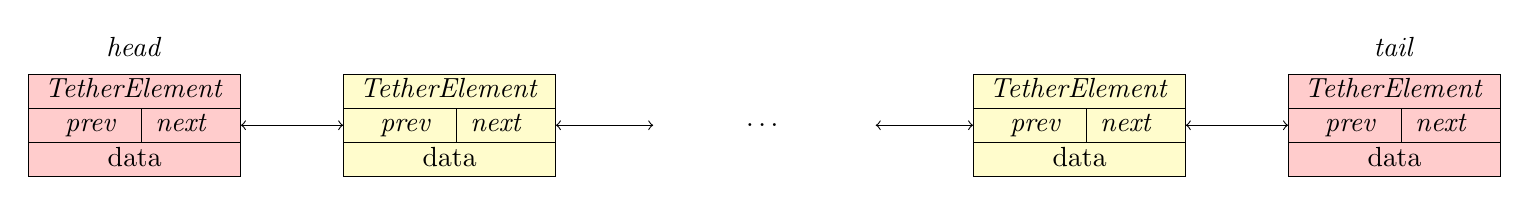
\begin{tikzpicture}
                \tikzset{TE/.style={draw, inner sep=0, outer sep=0, fill=yellow!20}}

                \node[TE, fill=red!20] (TE0) at (0,0) {\begin{tabular}{c} \textit{TetherElement} \\ \hline \hfill \textit{prev} \hfill \vline \hfill \textit{next} \hfill \\ \hline data \end{tabular}};

                \node[TE, fill=red!20] (TE4) at (16,0) {\begin{tabular}{c} \textit{TetherElement} \\ \hline \hfill \textit{prev} \hfill \vline \hfill \textit{next} \hfill \\ \hline data \end{tabular}};

                \foreach \i in {1,3} {
                    \node[TE] (TE\i) at (4*\i,0) {\begin{tabular}{c} \textit{TetherElement} \\ \hline \hfill \textit{prev} \hfill \vline \hfill \textit{next} \hfill \\ \hline data \end{tabular}};
                }
                \node[minimum width=80] (TE2) at (8,0) {\dots};
                \foreach \i in {0,1,2,3} {
                    \pgfmathtruncatemacro{\next}{\i +1}
                    \draw[<->] (TE\i) -- (TE\next);
                }

                \node (head) at (0,1) {\textit{head}};
                \node (tail) at (16,1) {\textit{tail}};
            \end{tikzpicture}
        }
        \caption{Liste doublement chainée}
        \label{fig:doubly_linked_list}
    \end{figure}

    \begin{figure}[!htb]
        \centering
        \resizebox{0.50\textwidth}{!}{
            \begin{tikzpicture}
                \begin{class}[text width=6cm]{Tether}{0,0}
                    \attribute{+ element\_mass : double}
                    \attribute{+ element\_volume : double}
                    \attribute{+ element\_length : double}
                    \attribute{+ position\_first : numpy.ndarray}
                    \attribute{+ position\_last : numpy.ndarray}
                    \attribute{+ elements : list of \textit{TetherElement}}
                \end{class}
            
                \begin{class}[text width=6cm]{TetherElement}{8.5,0}
                    \attribute{+ mass : double}
                    \attribute{+ volume : double}
                    \attribute{+ length : double}
                    \attribute{+ position : numpy.ndarray}
                    \attribute{+ velocity : numpy.ndarray}
                    \attribute{+ acceleration : numpy.ndarray}
                    \attribute{+ previous : TetherElement}
                    \attribute{+ next : TetherElement}
                    \attribute{+ K\_p : double}
                    \attribute{+ K\_d : double}
                    \attribute{+ K\_i : double}
                    \operation{+ F\_p(self) : numpy.ndarray}
                    \operation{+ F\_b(self) : numpy.ndarray}
                    \operation{+ F\_f(self) : numpy.ndarray}
                    \operation{+ Ft\_prev(self) : numpy.ndarray}
                    \operation{+ Ft\_next(self) : numpy.ndarray}
                \end{class}
            
                \aggregation{Tether}{}{~~~n}{TetherElement}
            \end{tikzpicture}
        }
        \caption{Diagramme de classe UML des classes \textit{Tether} et \textit{TetherElement}}
        \label{fig:uml_class}
    \end{figure}

\subsection{Suivi d'angles normalisés}
    Un problème avec la représentation numérique de l'orientation des solides est qu'elle est souvent normalisée, et les valeurs sont ainsi ramenées dans l'intervalle $[-\pi; \pi]$. On ne peut donc pas avoir l'orientation absolue, c'est à dire l'orientation d'un solide en prenant en compte les eventuels tours qu'il aurait pu faire sur lui-même.

    Pour résoudre ce problème, l'\textsc{Algorithme}~\ref{algo:suivi_angle} de suivi d'angles normalisés a été implémenté. Il prends en paramètres l'angle normalisé ainsi que l'angle précédemment calculé, et il retourne la valeur de l'angle absolu. L'idée de fournir l'angle précédent est de pouvoir retourner le nouvel angle qui se trouve dans le même quadrant et aussi de pouvoir suivre les sauts d'angles. Ainsi on peut suivre l'orientation absolue de solides en rotation dans l'espace, en ne fournissant que des orientations relatives ramenées dans l'intervalle $[-\pi; \pi]$, et en gardant en mémoire la précédente orientation calculée.
    
    \begin{algorithm}[!htb]
        \SetKwInOut{Input}{Entrées}
        \SetKwInOut{Output}{Sorties}
        \Entree{$angle\_normalise$, $angle\_absolu$}
        \Sortie{$angle\_absolu$}
        \Deb{
            $offset \leftarrow (angle\_absolu - angle\_normalise + \pi ) \pmod{2\pi}$ \\
            $angle\_absolu \leftarrow angle\_normalise + 2\pi \cdot offset$ \\
        }
        \Retour{$angle\_absolu$}

        \caption{Suivi d'angle} 
        \label{algo:suivi_angle}
    \end{algorithm}

    La \textsc{Figure}~\ref{fig:suivi_angle} présente les résultats de l'\textsc{Algorithme}~\ref{algo:suivi_angle} avec une angle variant dans l'intervalle $[-3\pi; 3\pi]$. On voit sur la première sous-figure l'angle réel et l'angle ramené dans l'intervalle $[-\pi; \pi]$ avec la présence de saut d'angles. Avec cette méthode, on est capable de suivre l'évolution de l'angle et de supprimer cess sauts afin de retrouver l'angle absolu visible dans la deuxième sous-figure et calculé uniquement à partir de la connaissance de l'angle normalisé.

    \begin{figure}[!htb]
        \centering
        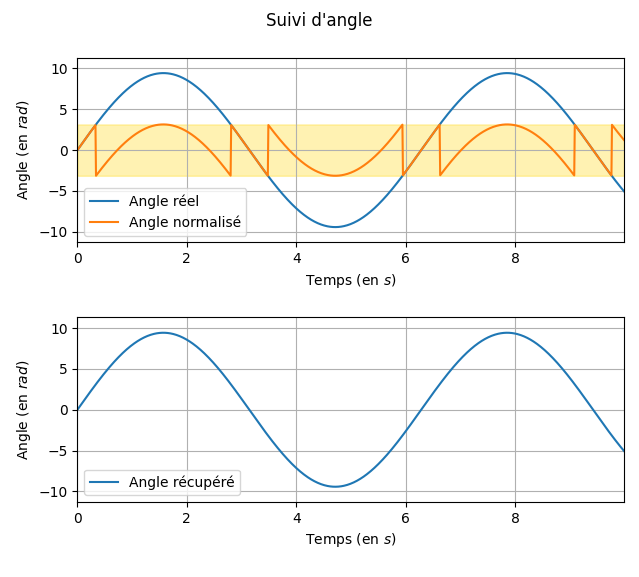
\includegraphics[width=0.5\textwidth]{suivi_angle.png}
        \caption{Suivi d'angle}
        \label{fig:suivi_angle}
    \end{figure}


\subsection{Resultats}

		\section{Simulation du garage d'Argos}

		\section{Simulation des structures sous-marines}
		